\input{configuration}

\title{Lecture 14 --- Buffering and Indexing }

\author{Jeff Zarnett \\ \small \texttt{jzarnett@uwaterloo.ca}}
\institute{Department of Electrical and Computer Engineering \\
  University of Waterloo}
\date{\today}


\begin{document}

\begin{frame}
  \titlepage

 \end{frame}
 

\begin{frame}
\frametitle{Buffering and Caching}

Buffering and caching are important in computing, as you surely know, since you have likely learned about it in multiple scenarios before now. 

The most recent probably related to caching in operating systems, where you may have modelled putting things into the L1 cache of a CPU. 

\begin{center}
	
\includegraphics[width=0.4\textwidth]{images/pfr.png}
\end{center}

 \end{frame}
 

\begin{frame}
\frametitle{Buffering and Caching}

It is, nevertheless, applicable to databases as well. 

Where before we were concerned about whether we needed to fetch a page from memory into cache. 

Now it is about whether we need to fetch a block from disk into memory.


\end{frame}

\begin{frame}
\frametitle{Buffering and Caching}

As discussed, a block number is used for a read or write operation, which we can translate into an address for the disk operation. 

Ideally, the block is found in the buffer, because that would be faster. 


\end{frame}

\begin{frame}
\frametitle{Buffering and Caching}


If the requested block is not there, we must load the block from disk, a very slow operation. 

Buffers are limited in size because memory is limited and it is expensive.

\end{frame}


\begin{frame}
\frametitle{Manage Carefully}
As you can imagine, we must manage the buffer carefully, just as cache has to be managed to figure out what blocks should be in it. 

The what will make the biggest difference is the replacement algorithm.

How we choose what blocks to be replaced is critical! 


\end{frame}


\begin{frame}
\frametitle{Manage Carefully}

That's a subject we know something about since we have already covered it in the operating systems course.

\begin{center}
	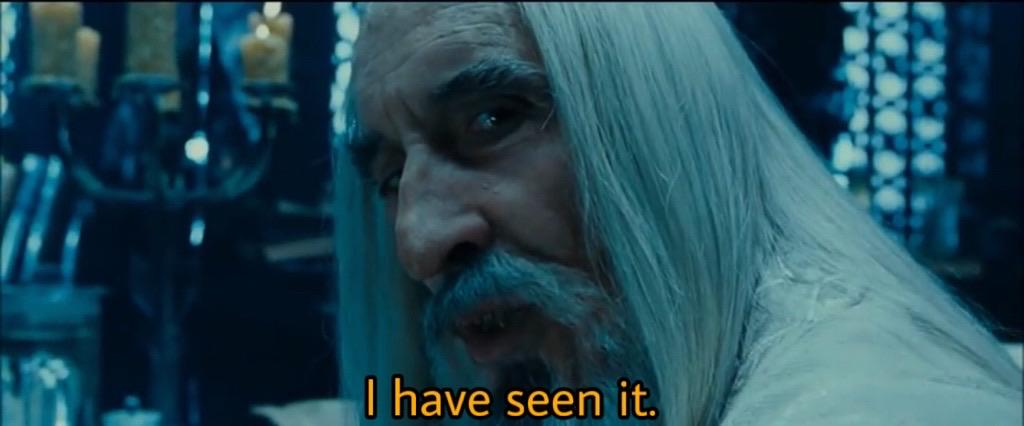
\includegraphics[width=0.6\textwidth]{images/seenit.jpg}
\end{center}

There are two considerations that change the scenario a little bit from the operating system view: pinned blocks and forced output of blocks.


\end{frame}

\begin{frame}
\frametitle{Pinned Blocks}

\alert{Pinned blocks} are necessary in the database: these are blocks that we do not allow to be written out to disk for some reason. 

The most common explanation for why disks cannot be written out to disk is that they are still being updated due to some transaction. 

Partial state should not be written to stable storage. 

\end{frame}

\begin{frame}
\frametitle{Forced Output}

\alert{Forced Output} of blocks is the mirror image of that; it's writing a block out to disk even though we do not need the space it's currently taking up. 

This is done to save the data to stable storage to minimize data loss in a crash.

\end{frame}


\begin{frame}
\frametitle{Now, Or Later?}

If a block has been altered in the buffer, then that change has to be written to disk at some point. 

It can be done immediately when the block is changed, or it can be done when the block is evicted from the buffer. 


\end{frame}


\begin{frame}
\frametitle{Now, Or Later?}

The second option means fewer main memory accesses, if a block is written to multiple times before it is sent to main memory. 

If a block has not been modified in buffer, it can simply be overwritten. 

If all other factors are equal, we should replace a block that has not been modified, as the work to write it out to memory need not be done.


\end{frame}

\begin{frame}
\frametitle{Replacement Algorithms}

The first approach to page replacement algorithms likely discussed was First-In-First-Out (FIFO). 

First-In-First-Out is quite easy to understand and implement. 

If there are $N$ frames, keep a counter that points to the frame that is to be replaced (the counter ranges from $0$ to $N-1$). 

Whenever a page needs to be replaced, replace the page at the counter index and increment the counter, wrapping around to 0 where necessary.

\end{frame}

\begin{frame}
\frametitle{Replacement Algorithms}

The least recently used (LRU) algorithm means the page that is to be replaced is the one that has been accessed most distantly in the past. 

You might consider time stamps and searching a list, but because there are only two operations, it need not be that complex. 

\end{frame}

\begin{frame}
\frametitle{Replacement Algorithms}

When a page in the cache is accessed, move that page to the back of the list. 

When a page is not found in cache, the page at the front of the list is removed and the new page is put at the back of the list. 

This requires nothing more than a cyclic doubly-linked list. 

\end{frame}

\begin{frame}
\frametitle{Best Algorithm}

Probably you have also learned that the LRU algorithm is the best choice. 

This is reasonable in an operating system, which uses the past accesses to predict the future. 

The database may be capable of making predictions about what it going to happen, allowing better results. 

\end{frame}

\begin{frame}
\frametitle{Best Algorithm}



\begin{center}
	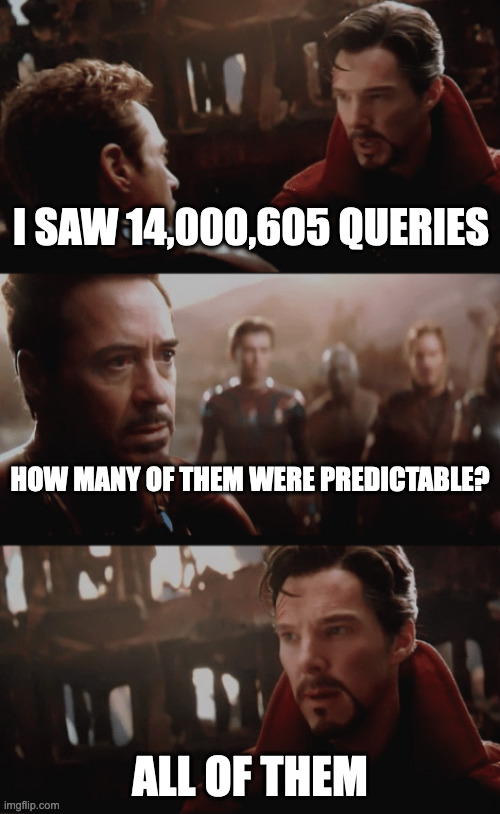
\includegraphics[width=0.35\textwidth]{images/predictable.jpg}
\end{center}

If the user requests an operation that will access all blocks of a record, we have a pretty good idea which ones we will want.

\end{frame}

\begin{frame}
\frametitle{I Want It All!}

Suppose then that there is a request for a select query that covers all tuples of a particular relation. 

Example: sum up the salaries of all the employees. 

To execute: examine every tuple once and only once. 

LRU would not be the best thing here!

\end{frame}

\begin{frame}
\frametitle{I Want It All!}

Once all the records in a block of the employee relation have been examined and added to the sum,  it can be replaced immediately. 

This is called the \alert{toss immediate} strategy.

\end{frame}

\begin{frame}
\frametitle{Join Me}

Now imagine that we need to do a join query, such as selecting from addresses joining with employees. 

Now, we need to consider each block of employees for a given address.

That is, after a block is used, it will not be needed again for a long time...\\
which is the opposite of the assumptions for the LRU strategy to make sense. 

So what should we do instead?

\end{frame}

\begin{frame}
\frametitle{I Want It Most!}
The answer is: MOST recently used (MRU). 

\begin{center}
	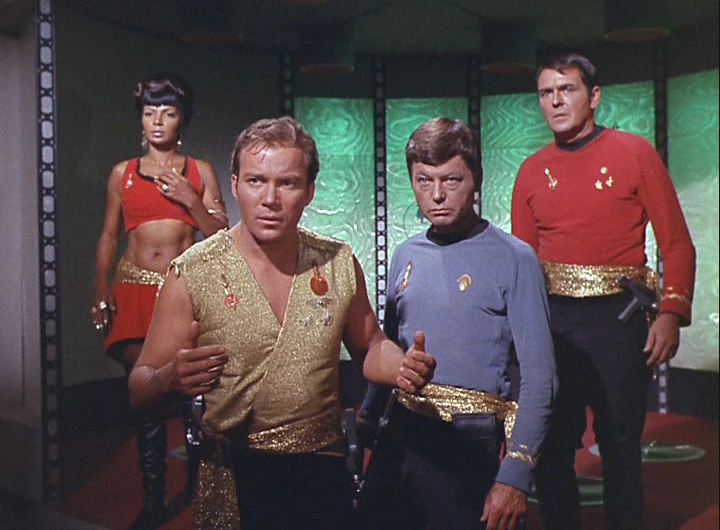
\includegraphics[width=0.4\textwidth]{images/mru.jpg}
\end{center}

When we are finished with a block, since we don't need it for a long time, we choose it for replacement.

This strategy must be combined with the pinning strategy so we do not evict from the buffer the block we are currently still working through.

\end{frame}


\begin{frame}
\frametitle{If I Have To...}

In addition to pinned blocks, there is also the forced output of blocks. 

Sometimes the crash recovery subsystem insists that certain blocks be written before the requested write can take place.

That is something that we will come to in the future. 

\end{frame}

\begin{frame}
\frametitle{Index Blocks}

Another small exception to our strategy for block replacement is index blocks. 

Since we will likely access the index frequently over the course of any operation, we want it to stay in memory. 

That does assume our query makes use of indices.

But the index blocks idea leads us into a discussion of the index in general.

\end{frame}

\begin{frame}
\frametitle{Indexing}

The concept of an index is familiar to anyone who has read a textbook or other large volume. 

\begin{center}
	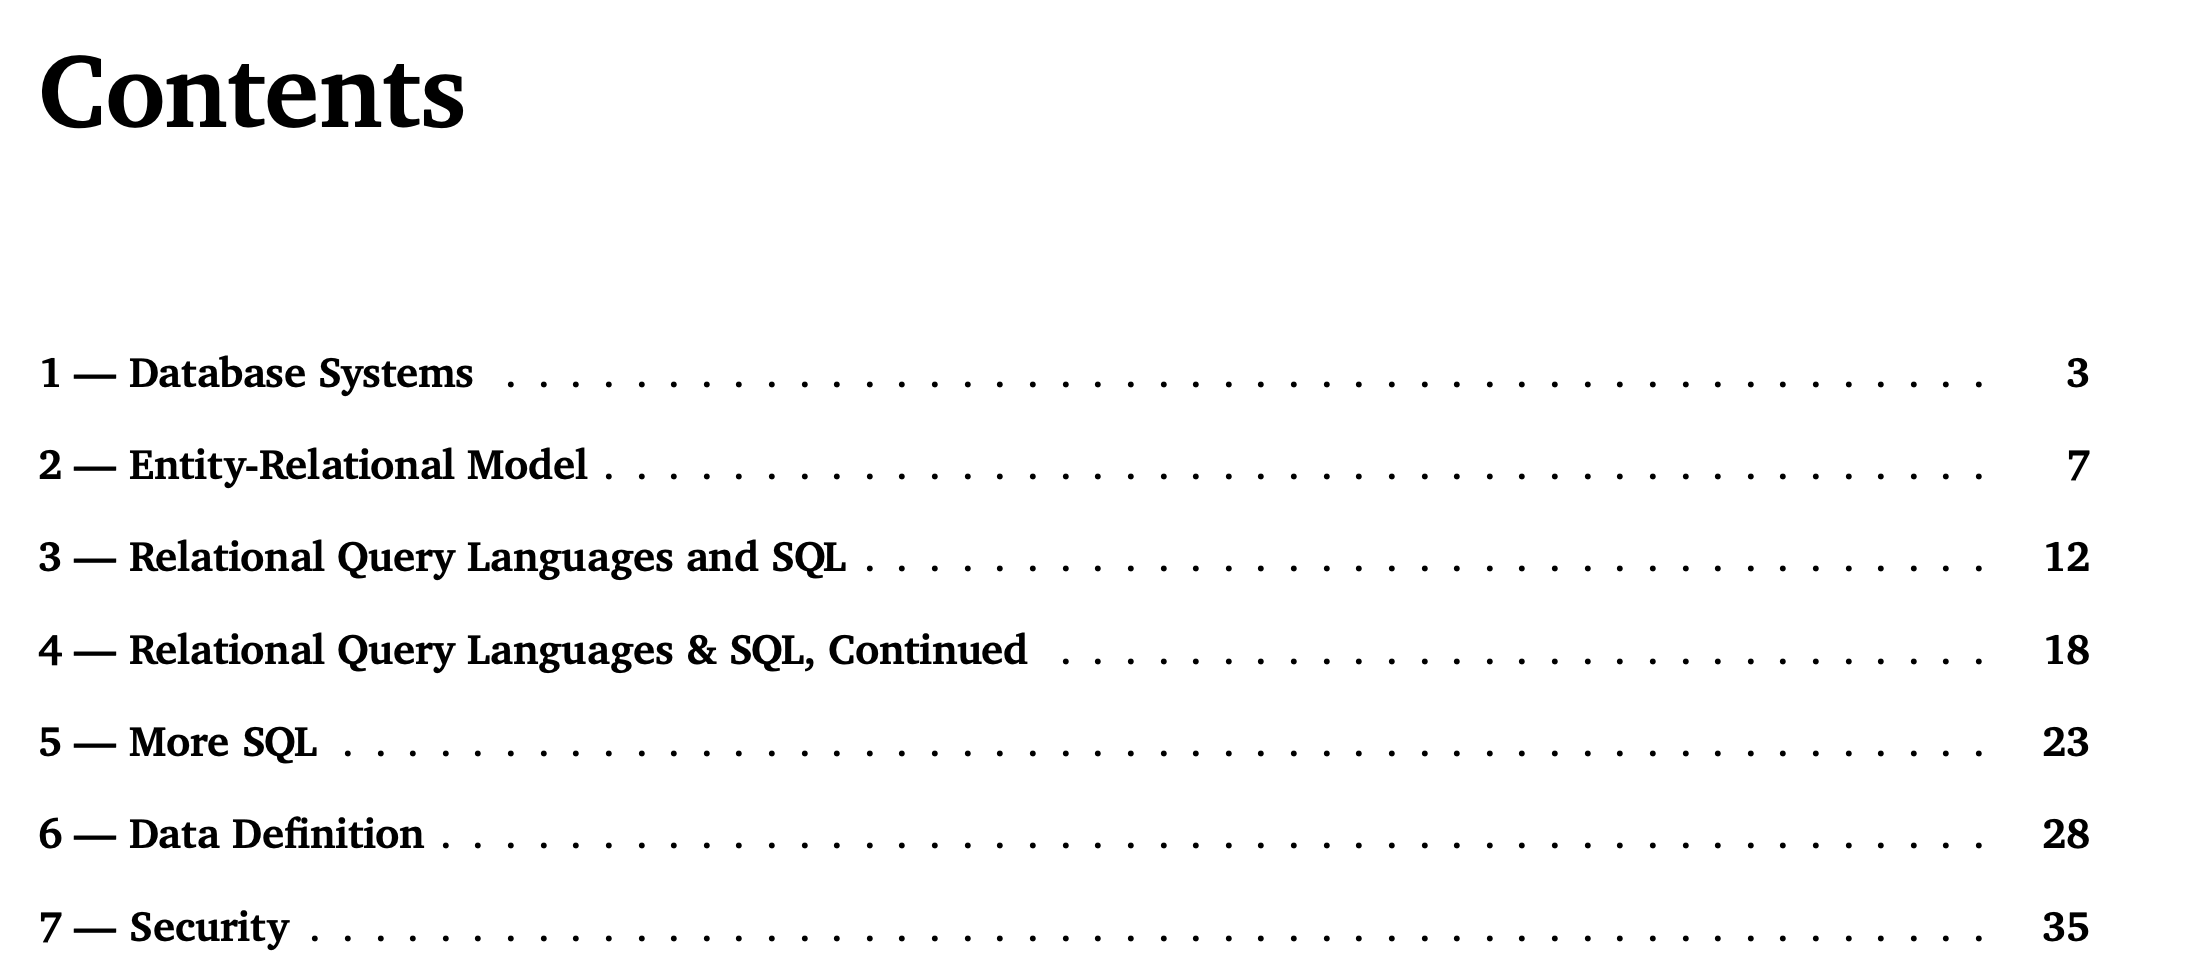
\includegraphics[width=\textwidth]{images/toc.png}
\end{center}


\end{frame}

\begin{frame}
\frametitle{Indexing}

At the beginning of the book there's an index (the ``table of contents'') and this can be used to quickly get to where you want to go in the book. 

 If this index did not exist then the only way to find what you were looking for is the hard way: search through the book until you reach that chapter.

\end{frame}


\begin{frame}
\frametitle{File Organizational Structure}

If the file already exists then it has some sort of organizational structure as we have previously discussed, even if that organization is no specific order. 

As we have already seen, if we want to find an record in such a file, we have no choice but to perform a linear search. 

The index saves us from doing that... if what we are looking for has an index.


\end{frame}

\begin{frame}
\frametitle{Do We Have an Index?}

Not all attributes in a relation will have an index, nor should they. 

Creating and maintaining an index takes significant work. 

And it makes sense to have an index for things we expect to search. 

\end{frame}

\begin{frame}
\frametitle{Do We Have an Index?}

If you are searching for a book, you can search by title or author, for example.

If you wished to search for books published in a certain year, say, 2016, and there is no index on that field?

We must scan the entire table to choose what tuples go in the result relation.
\end{frame}


\begin{frame}
\frametitle{We Do!}

Let's assume that the operation is on a field that has an index.

It can be kept sorted which means that it is quick to binary search the index and that tells us efficiently where we need to go to get to the desired record.

\end{frame}

\begin{frame}
\frametitle{Types of Index}

The \alert{primary index} is the ordering key field of an ordered file. 

This is the physical ordering of the file. 

If the ordering field is not unique, then a \alert{clustering index} is used instead (which makes this a clustered file). 

A \alert{secondary index} is an index on any field other than the one(s) used for ordering the file.

\end{frame}

\begin{frame}
\frametitle{Primary Index}

The primary index is a file itself, which itself is a listing of tuples. 

Each tuple contains the key \& address of the block where the data is stored. 

So if there is an address with id \texttt{24601} and it corresponds to disk block $x$ then the entry for this in the index is $<24601, x>$. 

\end{frame}

\begin{frame}
\frametitle{Primary Index}

One question we will face is whether every single tuple in the relation should have an entry in the index. 

If we choose yes, it is called a \alert{dense index}. 

Otherwise it is called a \alert{sparse index}. 

A sparse index has relatively fewer entries which means searching it is faster to search and operate on. 


\end{frame}

\begin{frame}
\frametitle{Sparse Index}

Find the index entry with the largest search key value that is less than or equal to the value we are looking for. 

Then we go to the record pointed to by that index entry and then search in that block until we find a match (or can conclude that there is no match). 

\end{frame}

\begin{frame}
\frametitle{Sparse Index}

This has the advantage that the index file is significantly smaller, but it will be slower to return an empty result if we do not find the value sought.

It does mean there are not as many entries that all point to the same block.

\end{frame}

\begin{frame}
\frametitle{Dense vs Sparse Index}
Dense index (left) and sparse index (right) in on the same data is shown below:

\begin{center}
\includegraphics[width=0.49\textwidth]{images/dense-index}
\includegraphics[width=0.49\textwidth]{images/sparse-index}
\end{center}

\end{frame}


\begin{frame}
\frametitle{Clustering Indexes}

Suppose instead that records are ordered on a non-unique field. 

That means there is a clustering index and the clustering index is a lot like a sparse index. 

There is an entry for each of the distinct values of the ordering field. 

To avoid the problem of insertion and deletion, one might have a block (or several) for each of the unique values of the ordering field.


\end{frame}

\begin{frame}
\frametitle{Secondary Index}

A secondary index, by definition, does not map to the order of the file. 

An index can be created on a unique field or a non-unique field and this, unlike clustering, is encouraged. 

As always, the index has two fields, the the indexing field and a block pointer (or record pointer). 

\end{frame}

\begin{frame}
\frametitle{Secondary Index}

If a secondary index is on a unique field, there is one index for every record in the data file and the secondary index will be dense. 

We cannot leave things out, because the file is not ordered based on the attributes being sought.
\end{frame}

\begin{frame}
\frametitle{Secondary Index}

\begin{center}
\includegraphics[width=0.6\textwidth]{images/secondary-index}
\end{center}


\end{frame}

\begin{frame}
\frametitle{Secondary Index, Nonunique Field}

A secondary index does not have to be on a unique field.

\begin{enumerate}
	\item \textbf{Duplicate entries}
	\item \textbf{Variable-Length Entries}	
	\item \textbf{Two-Level Index}
\end{enumerate}


\end{frame}

\begin{frame}
\frametitle{Two-Level Index}

\begin{center}
\includegraphics[width=0.65\textwidth]{images/secondary-index-2level}
\end{center}


\end{frame}



\begin{frame}
\frametitle{Multiple Levels}

Regardless of what implementation is used, operating on a secondary index is slower than operating on a primary index. 

That's okay, because it is still much better than not having an index at all, which would force linear searching. 

The secondary index has provided quick introduction to the idea of an index with multiple levels.

\end{frame}


\begin{frame}
\frametitle{Updating an Index}

Regardless of the type of index, whenever a record is inserted or deleted, the index needs to be updated. 

If an update affects an indexed field, then it must also be updated. 

Calling back to updating a relation, an update can be modelled as a deletion and an insertion.

Thus, we don't need to consider update separately.

\end{frame}


\begin{frame}
\frametitle{Insertion, Dense Index}

\begin{enumerate}
	\item If the search key does not appear in the index, insert an index entry at the appropriate position.
	\item If the search key is found then:
		\begin{enumerate}
			\item If the index stores pointers to all records with the same search key value, add a pointer to the new record in the index entry.
			\item Otherwise the index entry stores a pointer to the first record with that value; place the record being inserted after the other records with the same key.
		\end{enumerate}
\end{enumerate}


\end{frame}

\begin{frame}
\frametitle{Insertion, Sparse Index}

\begin{enumerate}
	\item If a new block is created, insert the first search key value from the new block into the index.
	\item Otherwise, no new block is created and:
		\begin{enumerate}
			\item If the new record is the lowest record in the block, update the index entry for that block.
			\item If the new record is not the lowest, no change to the index occurs.
		\end{enumerate}
\end{enumerate}

\end{frame}

\begin{frame}
\frametitle{Deletion, Dense Index}


\begin{enumerate}
	\item If the deleted record was the only one with its value, delete that search key from the index.
	\item Otherwise:
		\begin{enumerate}
			\item If the index stores pointers to all records with the same search key value, delete the pointer to the deleted record.
			\item Otherwise: if the deleted record is the first in the group, update the pointer to be the next item; if it is not then there is no change to make.
		\end{enumerate}
\end{enumerate}

\end{frame}


\begin{frame}
\frametitle{Deletion, Sparse Index}

\begin{enumerate}
	\item If the index does not contain an entry with the deleted value, there is nothing to change.
	\item Otherwise:
		\begin{enumerate}
			\item If the deleted record is the only one with its search key, replace it with the next search key and record pointer; unless that is already in the index, in which case just delete the entry.
			\item If it is not the only one with its search key, then update the pointer to point to the next record with that same value.
		\end{enumerate}
\end{enumerate}


\end{frame}

\begin{frame}
\frametitle{Next Steps}

These algorithms are generally extensible to multi-level indexes as well. 

\begin{center}
	
\includegraphics[width=0.5\textwidth]{images/deeper.jpg}
\end{center}

Update the lowest level index and the changes will cascade upwards if needed. 

\end{frame}

\begin{frame}
\frametitle{Next Steps}

From the point of view of the second level, the lower level is the same as if it is a file containing records. 

But, as we will see, this is something we are about to examine...


\end{frame}


\end{document}

